Hardware-in-the loop (HIL) simulation allows designers to test aspects of the running system using the data interfaces that would be presented to the actual physical device to be controlled (as much as possible) .  Fig. \ref{fig:sim_flow} shows our proposed overall development process for rapidly getting a system working with respect to actual hardware interfaces. The process starts with a fully simulated model, and progresses through steps where simulated elements are incrementally replaced by real implementations, resulting in a fully implemented system. The key idea is that interfaces are preserved throughout, and consistent interface semantics and behavior are maintained across the steps.

\begin{figure}[ht]
\centering
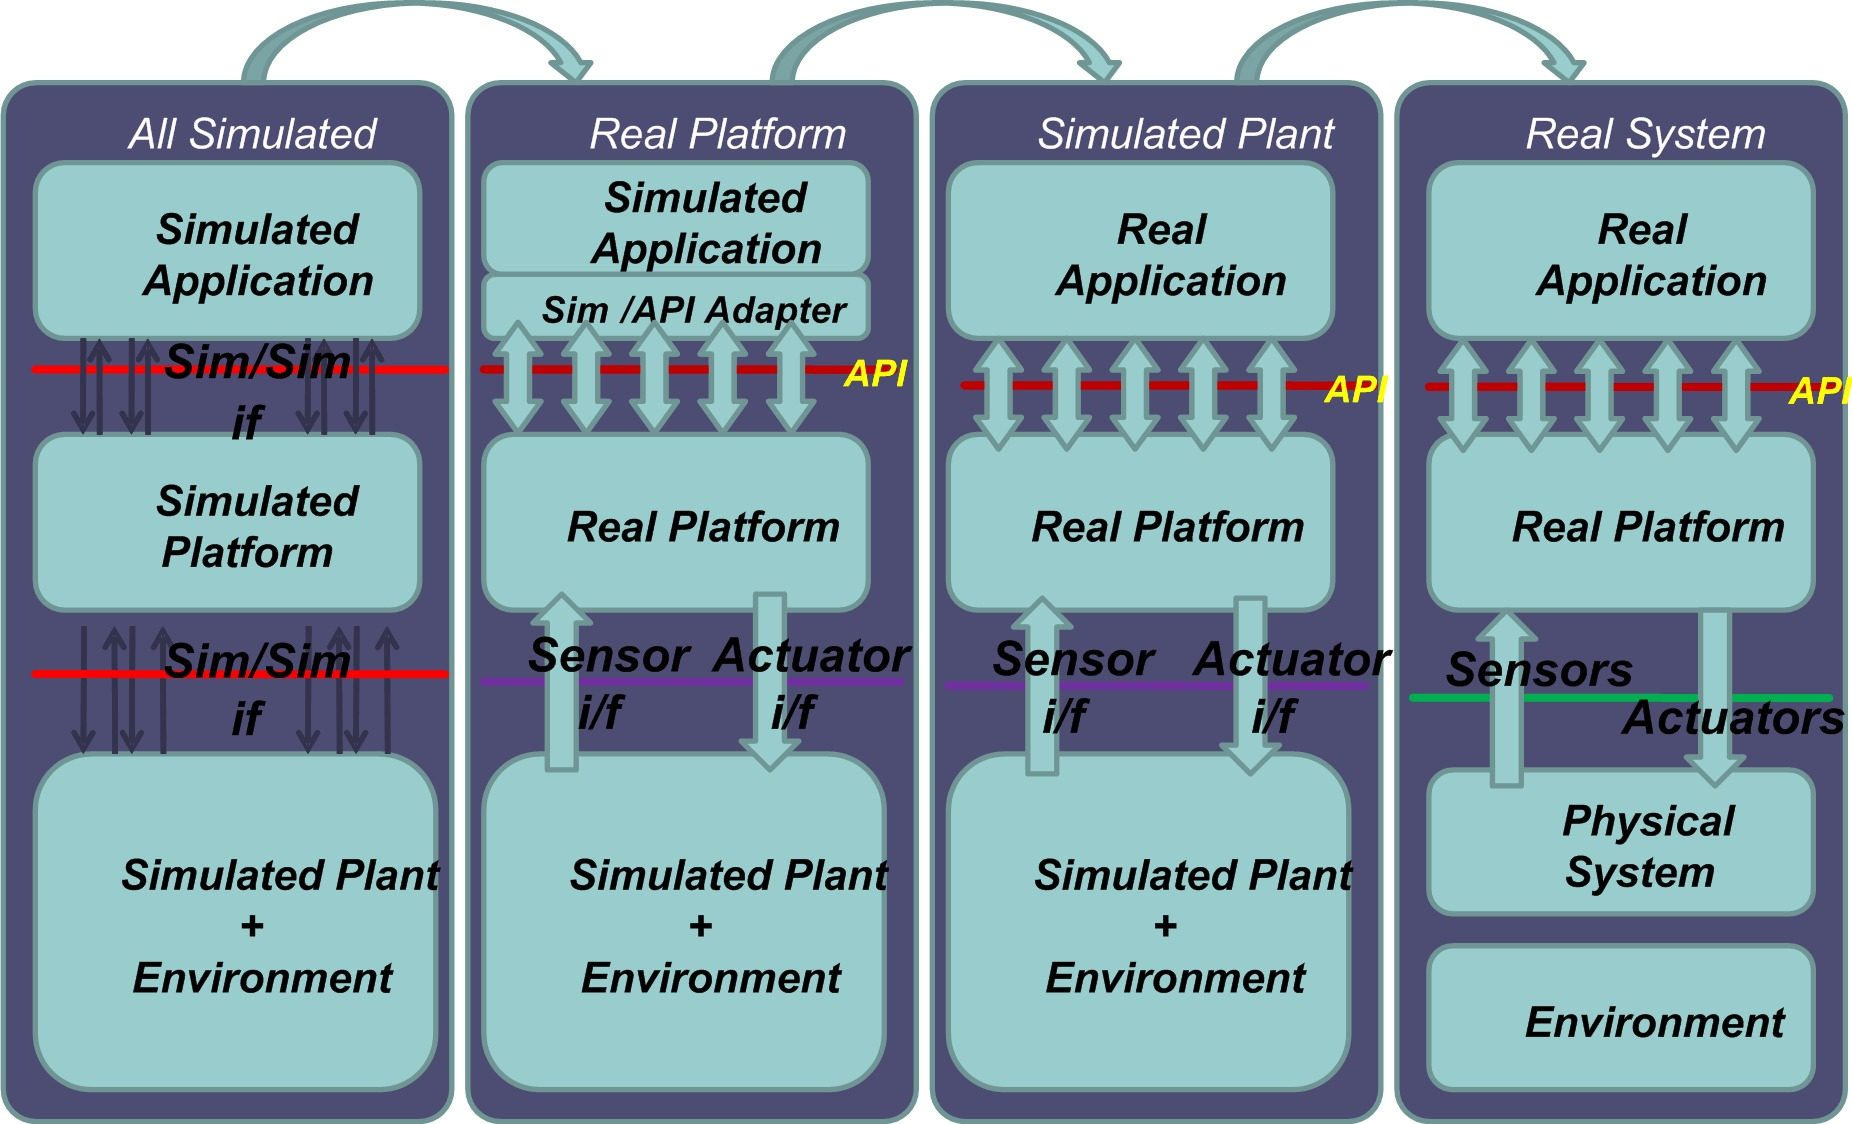
\includegraphics[width=\columnwidth]{figures/sim_flow.jpg}
    \caption{Proposed development process supported by hardware-in-the-loop simulation}
    \label{fig:sim_flow}
\end{figure}

The Mathworks' xPC Target\textregistered tool\cite{mathworks:tools} enables real-time HIL simulation of a model built in Simulink.  The HIL simulation model can be derived from the original (vehicle) simulation model, as shown in Fig. \ref{fig:xpc_sim}. Simulated dynamic systems (plants) must use fixed-step solvers only, and include explicit rate transition blocks where the data rate changes between blocks or subsystems.  Data transfers between the simulated plant and the Robostix controller occur on a serial link which acts as the 'sensor/actuator interface'.  This is a realistic simulation of the physical world, as the actual sensor devices also provide data via serial transfers.  In the figure the control subsystems have been removed and replaced by a block implementing data transfers (upper half). The lower half of the diagram has details for the transfer block and the message marshalling/unmarshalling functions. 

Our initial effort focused on quickly getting from models to a functional system. We used a simplified version of the dynamics to work out the communication and data interface details.  As such, we lack detailed results for performance, reliability, and safety of the generated controllers. However, some useful observations are in order:

\begin{enumerate}
\item Schedule determination attempts to enforce timing restrictions between sensors and actuators, as specified by the designer.  These specifications may be incomplete or infeasible.  The HIL simulation allowed us to quickly see destabilizing schedule effects, allowing us to debug and then validate the schedule.  TrueTime resimulation can also be useful in this regard, but it is less mature in our tools than the HIL simulation.  Our scheduling is not yet fully automated, as hand-tweaking is often necessary.
\item The HIL configuration effectively exposed the lack of synchrony between the sensors and the precisely timed control calculations.  We were forced to add smart buffering code to our virtual machine to ensure that serial transfers from the sensors had completed before attempting to use the data.
\end{enumerate}
